\newpage
\subsection{Resultados}

\label{subsection:resultados}
	tablas, gráficos, análisis y recomendaciones
	\begin{itemize}
		\item Aca debería explicar como fueron procesados los
                  resultados y que tipo de resultados se van a mostrar (ej. los
                  que tuvieron mejor y peor performance). \JS{hay que empezar a
                  poner cuales se van a mostrar y discutir}
                \item \JS{Baseline. Comparar con Wang}
		\item Resultados de dataset con imagenes reales.
		\begin{itemize}
			\item Se presentan los mejores resultados y los parámetros con los cuales se obtuvieron. Se van a presentar los gráficos de los 2 mejores resultados junto con sus matrices de confusión.
			\item Idem pero con los peores resultados obtenidos.
		\end{itemize}
		\item Idem con dataset sintéticos
		\item Idem con dataset sintéticos + reales.

	\end{itemize}
	
	Existen ciertas condiciones por las cuales no se pueden reproducir de manera exacta los resultados obtenidos por Wang et al. en \cite{wang}. La más importante es que el lenguaje usado para implementar el clasificador en el presente trabajo es Python, mientras que los autores usan matlab por lo cual pueden haber ciertas cosas que modifiquen los resultados. Otra de las razones es que en su trabajo no explican de manera clara y concisa el método que utilizan para binarizar los vectores, por lo cual en este trabajo se proponen $4$ métodos alternativos. La última razón tiene que ver con la aparente diferencia en la implementación de la función hog. La implementación en \cite{wang} es la de Piotr Dollar el cual está basado en \cite{DT05}. En este trabajo se usa una implementación obtenida de la libreria scikit-image la cual está basada tambien en \cite{DT05}. Sin embargo, si bien ambas funciones se basan en el mismo trabajo realizado por Dalal \& Triggs, existen ciertas diferencias.
	
	Ante esta situación se decide por establecer como baseline el resultado obtenido por la configuración más cercana a la usada por los autores en \cite{wang}. Los parámetros usados fueron: $8$ orientaciones y $6$ celdas por bloque para la función HOG; el valor de la longitud de los vectores de características fue establecido en $1536$ y usaron grupos de $6$ bits. En cuanto a la binarización de los vectores, si bien no hay un método concreto, basádo en el código provisto por los autores se pudo deducir que generaban números aleatorios entre $0$ y $1$ para armar el umbral. Para intentar acercarnos lo más posible a esa implementación, se decidió por usar el método bootstrap para afrontar el problema ya que es la función que más se apega a lo que hicieron. Por último, el valor de alpha surge de lo explicado en \ref{subsection:ferns} y es un valor que no está explicitado ni en el paper ni en el código de manera clara. La siguiente tabla muestra los valores luego de calcular la media sobre $5$ experimentos corridos sobre imágenes reales y sintéticas con los parámetros explicados anteriormente. Estos valores van a ser nuestros baselines a superar durante los siguientes experimentos.
	
	\begin{table}
		\centering
	    \begin{tabular}{ | l | l | l | p{5cm} |}
    			\hline
    				\textbf{Implementación} & \textbf{Score} \\ \hline
    				NATIVE+FERNS & 0.42\% \\ \hline
    				SINT+FERNS & 0.34\% \\
    			\hline
    		\end{tabular}	
    		\caption[Resultados reales y sintéticas para baseline]{Resultados obtenidos al acercarnos a la implementación de Wang et al.}
    		\label{table: Baseline}
	\end{table}
	 
	Esta subsección está dividida en tres partes. La primera corresponde a los resultados obtenidos de haber entrenado y evaluado el clasificador Random Ferns con imágenes de caracteres en escenas naturales. Los gráficos mostrados en esta parte reflejan la relación entre la dimensión de los grupos y la precisión del clasificador. En las dos subsecciones siguientes la relación pasará a ser entre la precisión del clasificador en relación a la cantidad de imágenes sintéticas por clase.
	
	La segunda etapa contiene los resultados de haber reemplazado el conjunto de prueba de imágenes reales por un conjunto de imágenes sintéticas (ver \ref{subsubsection:recon-caracteres}). El objetivo es demostrar como influye en la performance de clasificación el entrenar al clasificador con imágenes sintéticas.
	
	En la última parte, se procederán a mostrar los resultados de haber modificado al conjunto de entrenamiento de la primera parte agregándole en diferentes proporciones imágenes sintéticas. Se compara este último enfoque con los anteriores para ver el impacto que produce en la performance dicho cambio.
	
	A continuación, se puede observar en la tabla \ref{table: Wang paper} los resultados obtenidos por los autores del paper ``End-to-end scene text recognition'' tanto para sus experimentos con imágenes reales como con imágenes sintéticas. En la misma, \textit{NATIVE+FERNS} hace referencia a entrenar al clasificador Random Fern con imágenes nativas o reales. De la misma forma, \textit{SINT+FERNS} hace alusión a entrenar el mismo clasificador con imágenes sintéticas. Estos resultados si bien no constituyen un baseline válido ya que los experimentos son diferentes, están para reflejar la diferencia entre ambas implementaciones.
	
	\begin{table}
		\centering
	    \begin{tabular}{ | l | l | l | p{5cm} |}
    			\hline
    				\textbf{Implementación} & \textbf{Score} \\ \hline
    				Wang NATIVE+FERNS & 0.54\% \\ \hline
    				Wang SINT+FERNS & 0.47\% \\
    			\hline
    		\end{tabular}	
    		\caption[Resultados reales y sintéticas de Wang]{Resultados obtenidos por Wang et al. en \cite{wang}}
    		\label{table: Wang paper}
	\end{table}

	\subsubsection{Imágenes Reales}
	
	En esta parte se van a mostrar cinco gráficos. Los primeros 4 corresponden a los métodos utilizados en la binarización con lo cual se busca ver cual de los 4 arroja mejores resultados. Además, los primeros cuatro resultados reflejan la diferencia en performance al considerar grupos de diferente dimensión $\in \{ 1, 2, 4, 8, 10, 12\}$. Con esto buscamos establecer para cada caso, qué dimensión arroja los mejores resultados. Cabe aclarar que cada gráfico refleja la media de los resultados de 5 corridas del experimentos junto con la desviación estandard asociada. El quinto gráfico \ref{fig: Reales-Comparativa metodos} reune los mejores resultados de clasificación de los cuatro primeros, para establecer una comparación más precisa. La tabla \ref{table: reales-comparativa} se muestra un resumen de los mejores valores.
	
	 Dada la gran cantidad de parámetros que se manejan en estos experimentos, se va a intentar dejar detallado en el análisis cuales son los mejores y se los va a usar para los siguientes experimentos.
		
			\begin{figure}[htbp!]
				\centering
				\subfloat[Resultados usando la media \label{fig: Reales-media}]{
					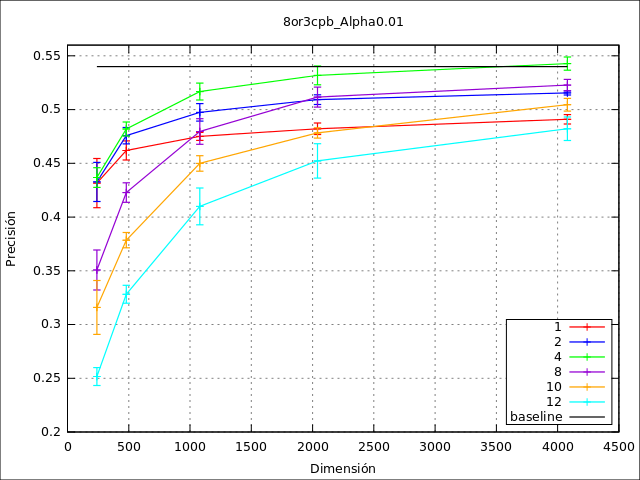
\includegraphics[width=8cm]{img/resultados/reales/mean.png}
				}
				\subfloat[Resultados usando la mediana \label{fig: Reales-mediana}]{
					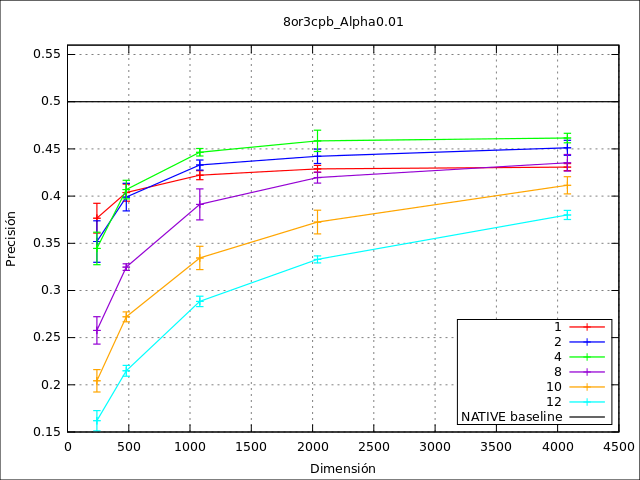
\includegraphics[width=8cm]{img/resultados/reales/median.png}
				}
				\\
				\subfloat[Resultados usando la distribución exponencial \label{fig: Reales-expon}]{
					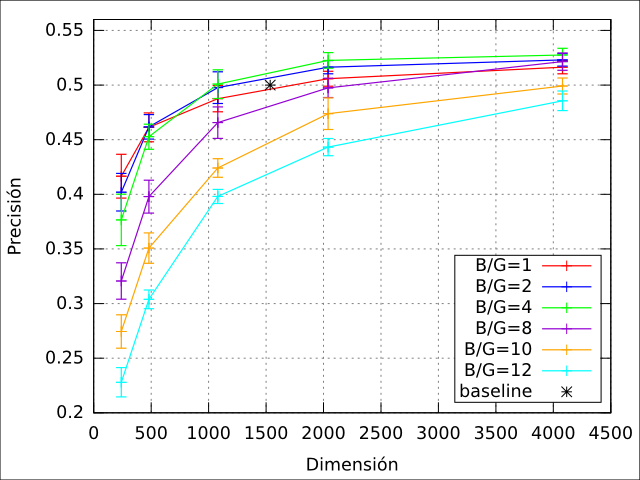
\includegraphics[width=8cm]{img/resultados/reales/expon.png}
				}
				\subfloat[Resultados usando bootstrap\label{fig: Reales-bootstrap}]{
					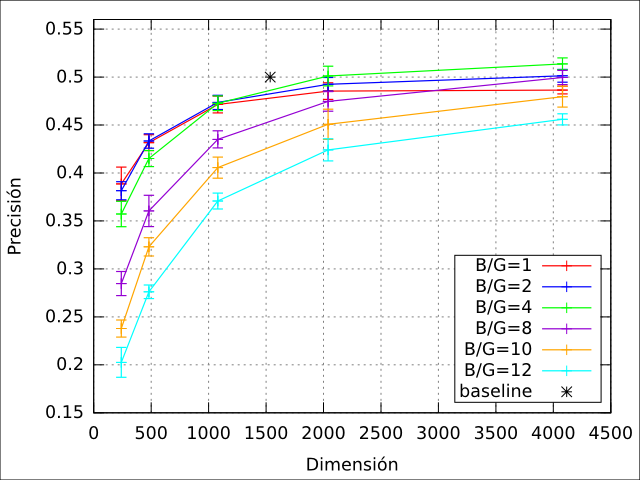
\includegraphics[width=8cm]{img/resultados/reales/bootstrap.png}
				}
				\caption[Resultados-Reales]{Esta figura presenta los resultados obtenidos por los 4 métodos propuestos para la binarización de los vectores.}
				\label{fig: Resultados-Reales}
			\end{figure}
			
	Teniendo en cuenta los resultados en \ref{fig: Resultados-Reales}, a simple vista se puede observar que los resultados obtenidos usando la media como método para binarizar los vectores son los mejores, llegando a un $54\%$ de precisión. En el caso opuesto, el usar la mediana arrojó los peores resultados ya que en el mejor de los casos se supera el $47\%$ a diferencia de bootstrap que llega a $51\%$ . El uso de la distribución exponencial en los casos donde la longitud de los grupos es baja ($1$, $2$ bits por grupo) supera a la media en performance pero se mantiene por debajo a medida que aumentamos este valor (casos $\{ 4, 8, 10, 12\}$ bits por grupo). Los valores que podemos encontrar en \ref{fig: Reales-expon} se acercan a los del a media llegando a un máximo en la precisión de $53\%$. En cuanto al uso de bootstrap, se puede apreciar que los resultados se mantienen por debajo de los obtenidos con la distribución exponencial y la media con puntajes que rondan entre $45\%$ y $52\%$.
	
	En cuanto a las dimensiones evaluadas $\{ 240, 480, 1080, 2040, 4080 \}$ es claro que a medida que aumentamos la longitud de los vectores aumenta la performance. Se puede ver que, cuando se usan vectores de longitud reducida (en este caso $240$), se marca una diferencia importante en la precisión entre los experimentos realizados con grupos de dimensionalidad baja $\{ 1, 2, 4 \}$ y alta $\{8, 10, 12\}$. Es decir, dejando fija la dimensión de los vectores en $240$, mientras más chico es el tamaño de los grupos mejor es el resultado (se puede observar en cualquiera de los gráficos en \ref{fig: Resultados-Reales}). En el otro extremo, si usamos grupos de $12$ bits la precisión baja bastante. La misma relación se mantiene a medida que aumentamos el tamaño de los vectores de características hasta cierto punto. Por ejemplo, en \ref{fig: Resultados-Reales} y específicamente en \ref{fig: Reales-media} es claro que a partir del uso de $1080$ como tamaño de vector en adelante, el uso de grupos de longitud mayor arroja mejores resultados. Lo mismo sucede en las otras figuras en diferentes puntos. En cuanto al uso del valor $4080$ como longitud del vector se puede notar como disminuye la brecha entre los valores de los resultados. \RC{Dar una razón por la cual esto pasa}.
	
	Otro parámetro a analizar aquí es \textit{alpha} $\in \{ 0.0001, 0.001, 0.01, 0.1, 1\}$. Los mejores resultados de cada método se dieron cuando el valor de \textit{alpha} se estableció en $0.01$ y son los que se muestran en la figura \ref{fig: Resultados-Reales}. Valores por encima $0.01$ o muy cercanos a 0 no llegaron en los experimentos a igualar la precisión obtenida con el valor de \textit{alpha} elegido. Por cuestiones de espacio se decidió mostrar en esta sección los resultados que se obtuvieron con el mejor valor de \textit{alpha}. El resto de los gráficos se pueden encontrar en el apéndice ``B'' con el resto de los resultados de los experimentos. \RC{Hacer apéndice B y explicar como influye alpha en los resultados}.
	
	Al igual que con el parámetro \textit{alpha}, hay $2$ parámetros que se dejaron fijos y son los relacionados con la función de HOG: la cantidad de \textit{orientaciones} y la cantidad de \textit{celdas por bloque}. Se decidió por usar $8$ y $9$ respectivamente ya que dichos valores devuelven los mejores resultados. Las razones por las cuales estos constituyen la mejor configuración escapa al análisis de este trabajo.
	
	
			\begin{figure}[htbp]
				\centering
				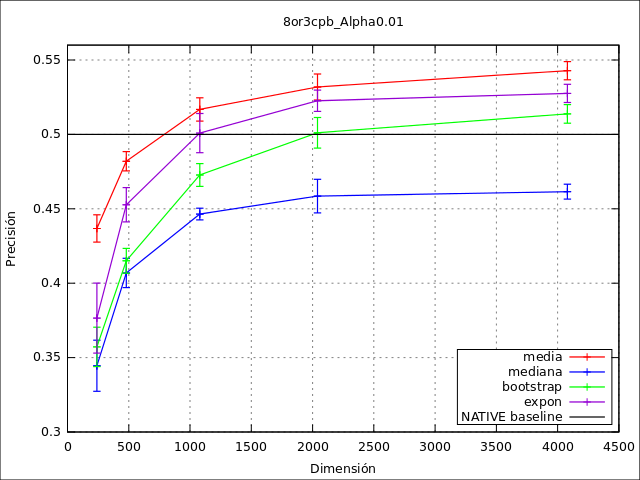
\includegraphics[scale=0.6]{img/resultados/reales/comparativa_metodos.png}
				\caption[Reales comparativa]{El gráfico muestra las mejores curvas de los gráficos presentados en la figura \ref{fig: Resultados-Reales} con la mejor configuración}
				\label{fig: Reales-Comparativa metodos}
			\end{figure}
	
	Del análisis realizado surge que la mejor configuración está dada por \textit{alpha = $0.01$}, \textit{orientaciones = $8$}, \textit{celdas por bloque = $9$}, \textit{bits por grupo = $4$} y \textit{dimensión del vector = 4080}. Se puede observar en \ref{fig: Reales-Comparativa metodos} las mejores curvas para cada método utilizando la mejor configuración (a excepción de la longitud del vector con el objetivo de ver la curva de crecimiento). Queda claro que la media se puede establecer como el mejor método para la binarización por lo cual en los próximos experimentos se procederá a trabajar con el mismo. De la misma manera la mediana termina siendo el peor método. De este último caso se puede ver que incluso para la mejor configuración tiene a ``aplanarse'' a medida que aumentamos la dimensión del vector característica
		
\newpage

	\begin{table}
		\centering
		\begin{tabular}{ | l | l | l | p{5cm} |}
    			\hline
    				\textbf{NATIVE + FERNS} & \textbf{Score} \\ \hline
    				Media & 0.54\% \\ \hline
    				Mediana & 0.47\%\\ \hline
    				Exponencial & 0.53\% \\ \hline
    				Bootstrap & 0.52\%\\ 
    			\hline
    		\end{tabular}
    		\caption[Resultados imagenes naturales]{Tabla comparativa entre los diferentes métodos propuestos para la binarización en la clasificación de caracteres en escenas naturales.}
    		\label{table: reales-comparativa}
    	\end{table}
    	
    	
    	\newpage
    	\subsubsection{Imágenes Sintéticas}
    	
    En esta etapa se procederán mostrar los resultados obtenidos de los experimentos con las imágenes sintéticas. Además, los gráficos van a representar la relación entre la cantidad de imágenes sintéticas por clase (dado por \textit{IPC} en las siguientes figuras) y la precisión de clasificación dada por los $6$ valores a evaluar que son las dimensiones de los grupos. Teniendo en cuenta los resultados anteriores con las imágenes reales, se decidió por trabajar $8$ orientaciones, $9$ celdas por bloque, alpha de $0.01$ y usando la media como método de binarización ya que son los parámetros que dieron los mejores resultados.
    
    Las figuras que se presentan a continuación están organizadas de la siguiente manera. Se van a presentar de manera continua el mejor y el peor resultado para cada experimento utilizando uno de los métodos de binarización. De la misma manera que se hizo para las imágenes reales, se va a incluir un gráfico con las mejores curvas de entre todos los gráficos presentados para que sea más fácil visualizar los mejores resultados.


			\begin{figure}[htbp]
				\centering
				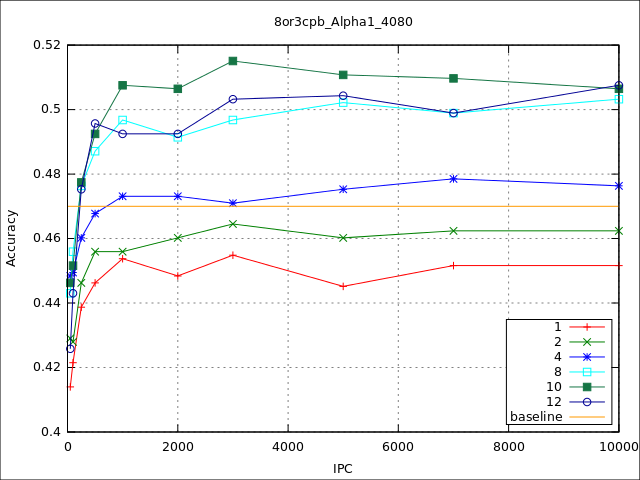
\includegraphics[scale=0.6]{img/resultados/sinteticas/best_media_8or3cpb_Alpha1_4080.png}
				\caption[Sintéticas media mejor resultado]{El gráfico muestra la configuración que devolvió los mejores resultados al utilizar la media en la binarización. Parámetros del mejor resultado: \textit{alpha:1}, \textit{IPC:3000}, \textit{dim grupo: 10}, \textit{dim vector: 4080}}
				\label{fig: Sinteticas-media-mejor}
			\end{figure}
			
			\begin{figure}[htbp]
				\centering
				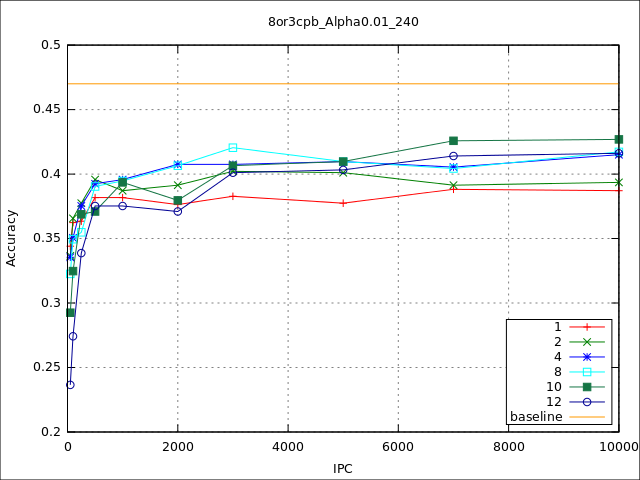
\includegraphics[scale=0.6]{img/resultados/sinteticas/worst_media_8or3cpb_Alpha0,01_240.png}
				\caption[Sintéticas media bajo resultado]{El gráfico muestra la configuración que devolvió los peores resultados al utilizar la media en la binarización. Parámetros del peor resultado: \textit{alpha:0.01}, \textit{IPC:50}, \textit{dim grupo: 12}, \textit{dim vector: 240}}
				\label{fig: Sinteticas-media-peor}
			\end{figure}
			
			\begin{figure}[htbp]
				\centering
				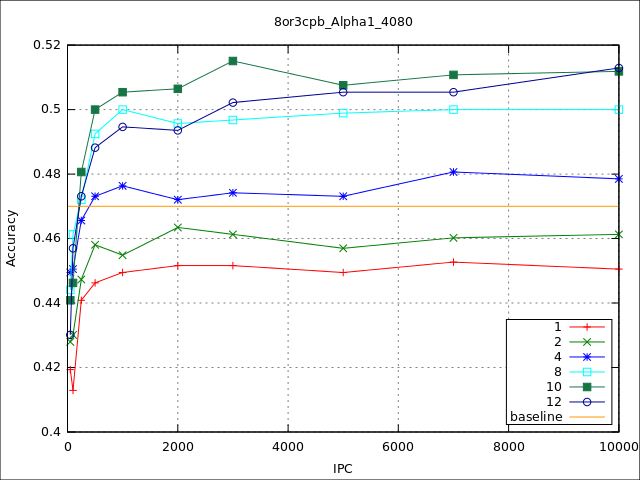
\includegraphics[scale=0.6]{img/resultados/sinteticas/best_expon_8or3cpb_Alpha1_4080.png}
				\caption[Sintéticas exponencial mejor resultado]{El gráfico muestra la configuración que devolvió los mejores resultados al utilizar la distribución exponencial en la binarización. Parámetros del mejor resultado: \textit{alpha:1}, \textit{IPC:3000}, \textit{dim grupo: 10}, \textit{dim vector: 4080}}
				\label{fig: Sinteticas-expon-mejor}
			\end{figure}
	
			\begin{figure}[htbp]
				\centering
				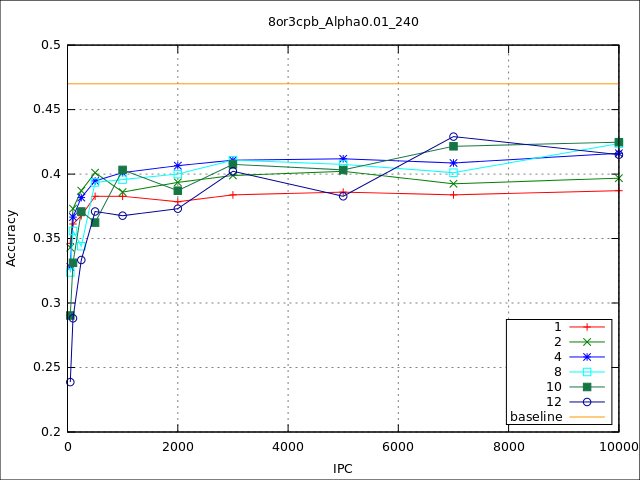
\includegraphics[scale=0.6]{img/resultados/sinteticas/worst_expon_8or3cpb_Alpha0,01_240.png}
				\caption[Sintéticas exponencial peor resultado]{El gráfico muestra la configuración que devolvió los peores resultados al utilizar la distribución exponencial en la binarización. Parámetros del peor resultado: \textit{alpha:0.01}, \textit{IPC:50}, \textit{dim grupo: 12}, \textit{dim vector: 240}}
				\label{fig: Sinteticas-expon-peor}
			\end{figure}
			
			
			\begin{figure}[htbp]
				\centering
				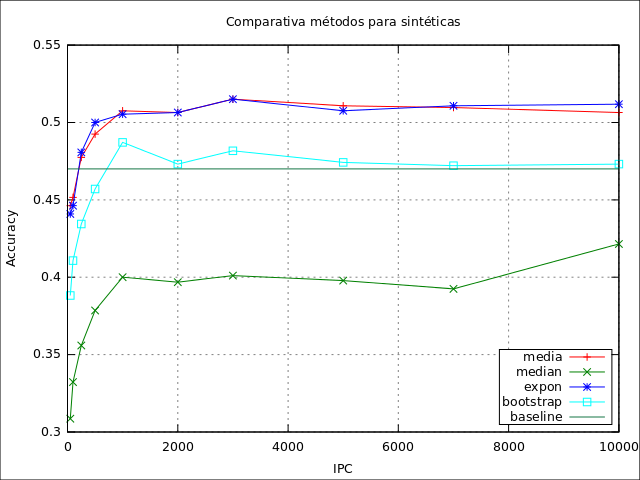
\includegraphics[scale=0.6]{img/resultados/sinteticas/comparativa_metodos.png}
				\caption[Sintéticas comparativa métodos]{El gráfico muestra las mejores curvas de los gráficos de cada método. \ref{fig: Sinteticas-media-mejor}~\ref{fig: Sinteticas-median-mejor}~\ref{fig: Sinteticas-expon-mejor} y \ref{fig: Sinteticas-bootstrap-mejor}}
				\label{fig: Sinteticas-comparativa metodos}
			\end{figure}

\newpage

	Hacer texto con las siguientes ideas
	\begin{itemize}
		\item En los experimentos con imágenes sintéticas en general a más cantidad de imágenes por clase mayor es la performance de clasificación. Sin embargo llega un punto en que se deja de aumentar la perfomances y en varios casos disminuye despues de cierto punto.
		\item Es claro que para este tipo de experimentos es mejor tener grupos de dimensiones mayores a los propuestos para las imágenes reales. Analizar que los casos donde los grupos tienen 12 bits la performance decae a comparación de los casos donde los mismo tienen 10 bits.
		\item Defenitivamente la mediana y bootstrap no son buenos métodos para binarizar.
	\end{itemize}

	\begin{table}
		\centering
		\begin{tabular}{ | l | l | l | p{5cm} |}
    			\hline
    				\textbf{SINT(1000) + FERNS} & \textbf{Score} \\ \hline
    				Media & 0.51\% \\ \hline
    				Mediana & 0.4\%\\ \hline
    				Exponencial & 0.5\% \\ \hline
    				Bootstrap & 0.49\%\\ 
    			\hline
    		\end{tabular}
    		\caption[Resultados imágenes sintéticas vs Wang]{Tabla comparativa entre el resultado obtenido por Wang para imágenes sintéticas y los obtenidos en el presente trabajo, utilizando los mejores resultados entre los cuatro umbrales propuestos. Se consideran para poder realizar la comparación los resultados cuando se evalua al clasificador con 1000 imágenes sintéticas.}
    	\end{table}
			
\newpage
    	\subsubsection{Imágenes Reales y Sintéticas}
    	
	Por último se van a mostrar los resultados correspondientes de haber entrenado al clasificador con conjuntos de entrenamiento mixtos. Se procederá a mostrar los gráficos con las mejores y peores configuraciones y sus resultados. También se mostrarán las matrices de correlación para todos estos casos. Teniendo en cuenta el análsis anterior, se van a mostrar los resultados de haber utilizado solamente la la media como umbral ya que fue la que retornó los mejores valores.
	
	El gráfico a continuación presenta el eje \textit{x} en escala logarítmica para poder apreciar mejor las variaciones que se dan al experimentar con valores cercanos entre sí.
	
			\begin{figure}[!htbp]
				\centering
				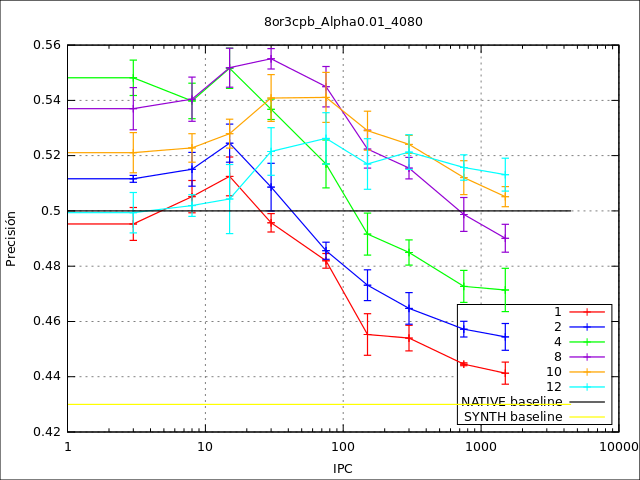
\includegraphics[scale=0.6]{img/resultados/mixtas/best_mean.png}
				\caption[Mixtas media mejor resultado]{El gráfico muestra la configuración que devolvió los mejores resultados.}
				\label{fig: Mixtas-media-mejor}
			\end{figure}

	De la figura \ref{fig: Mixtas-media-mejor} se puede desprender el siguiente análisis. El primero, y uno de los más importantes, hace referencia a la influencia en la clasificación de ir agregando de manera incremental imágenes sintéticas durante la etapa de entrenamiento. Se puede observar que a nivel general todos los experimentos llegaron a un punto donde su performance se desplomó al seguir agregando imágenes sintéticas en el entrenamiento. Sin embargo, este cambio ocurrio en diferentes momentos dependiendo del caso. Por ejemplo, cuando trabajamos con grupos de dimensionalidad baja ($1$, $2$ y $4$ bits por grupo), la precisión del clasificador va en aumento hasta que se llega a un máximo correspondiente al haber entrenado al sistema con igual cantidad de imagenes reales y sintéticas. A partir de ese punto el seguir incrementando la proporción de sintéticas sobre reales trajo efectos negativos en los resultados como se puede apreciar en el gráfico presentado. En los casos donde consideramos $10$ y $12$ bits por grupo el rendimiento se desploma cuando consideramos más de 75 imágenes sintéticas. La mejor curva en el gráfico la obtenemos cuando consideramos $8$ bits por grupo y entrenamos al clasificador con el doble de imágenes sintéticas que reales. Este resultado difiere con respecto al análisis realizado para los experimentos con imágenes reales donde consideramos que el mejor parámetro era considerar grupos de $4$ bits. En la mayoría de los casos se dan buenos resultados cuando la cantidad de imágenes sintéticas sobre las reales es la misma ($1$, $2$ y $4$) o se duplica ($8$ y $10$).
	
	Una de las diferencias con los análisis realizados en los experimentos con imágenes reales, es que el mejor resultado se encuentra cuando se usan grupos de $8$ bits. 


			\begin{figure}[!htbp]
				\centerline{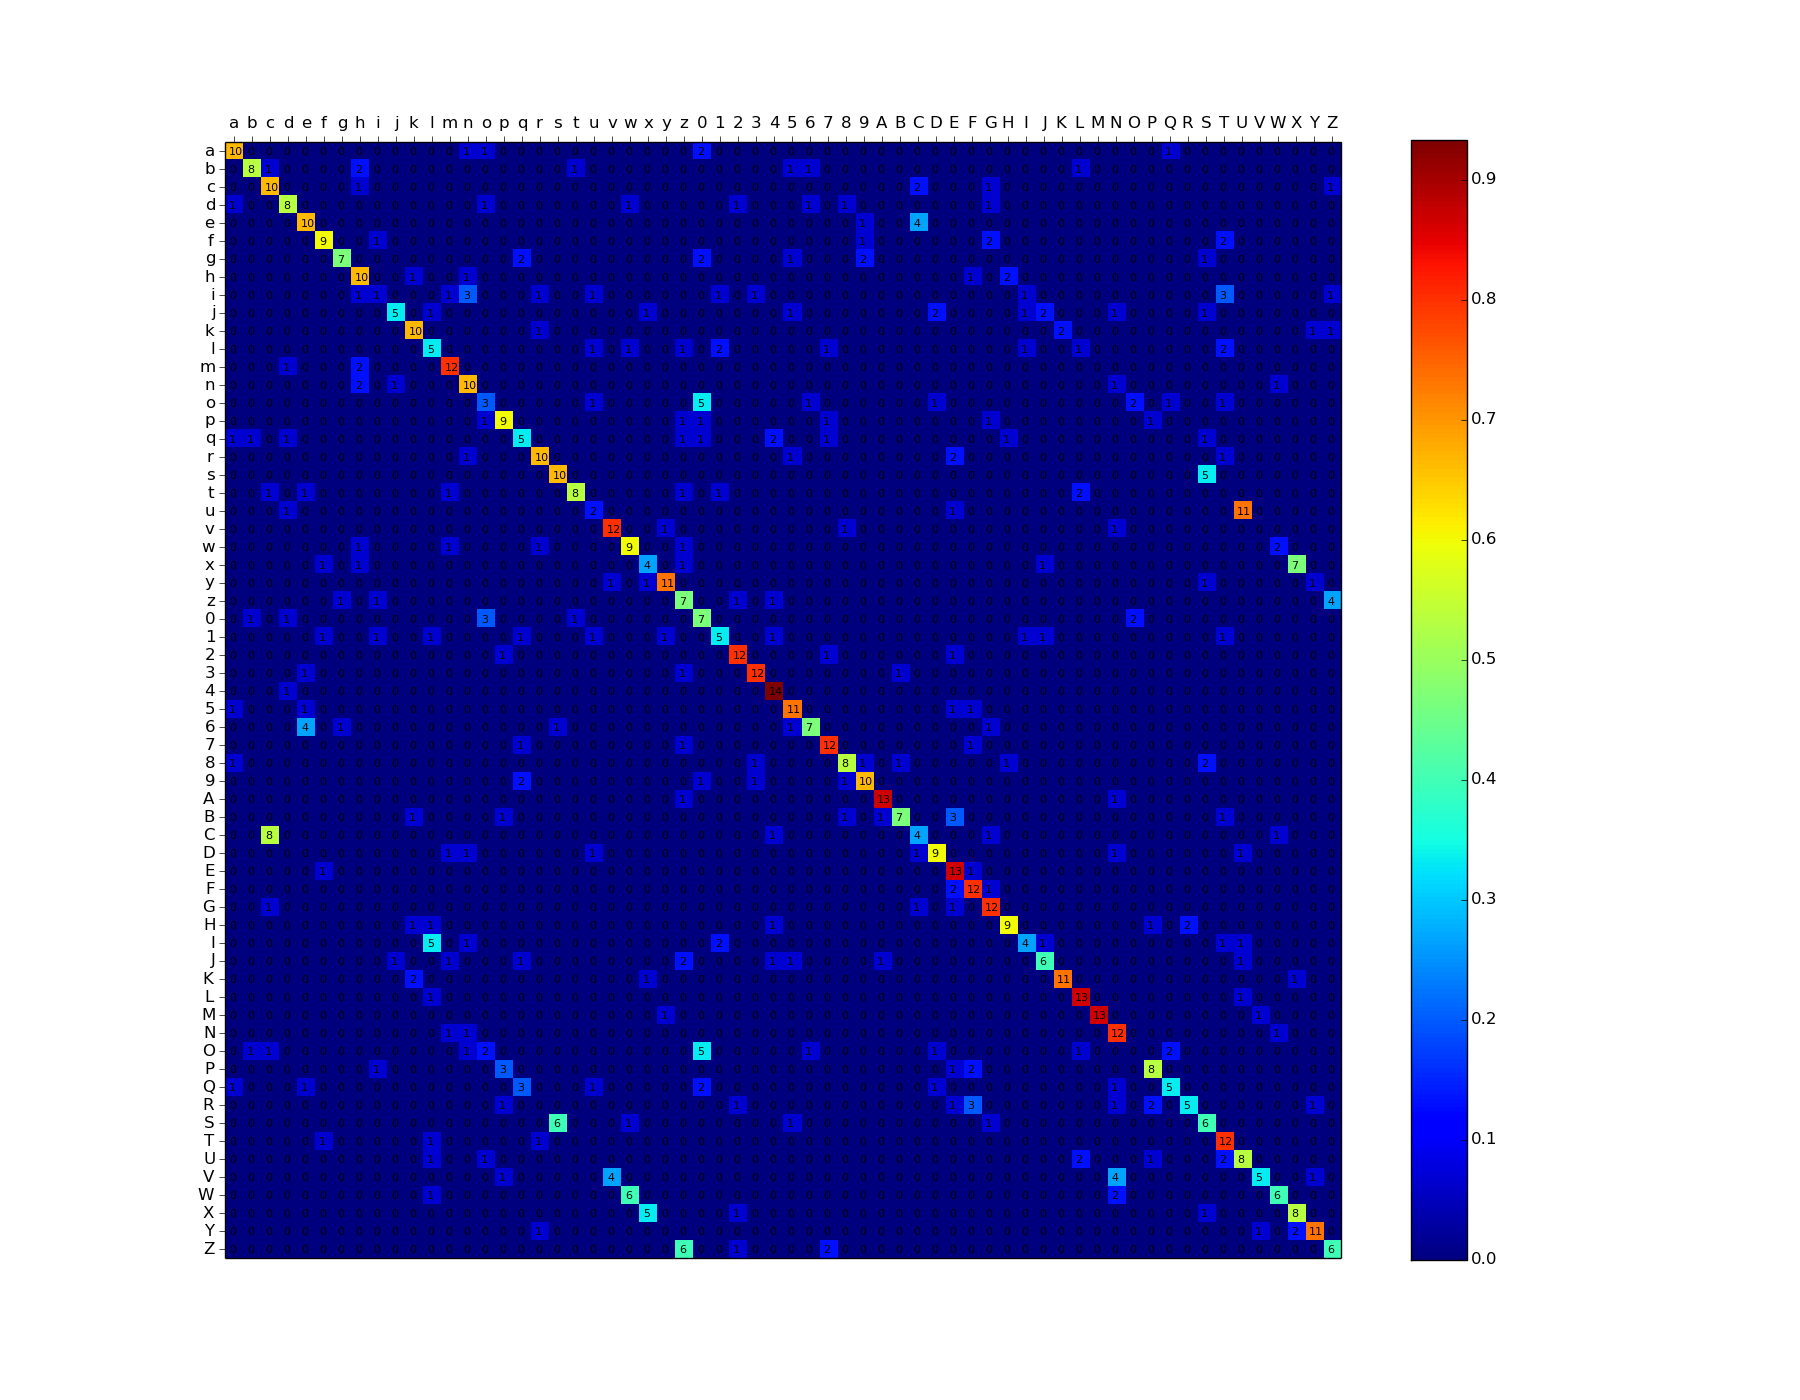
\includegraphics[scale=0.4]{img/resultados/mixtas/best_mean_matrix_Alpha0,01_4080-8.png}}
				\caption[Mixtas Matriz expon]{Matriz de correlación del gráfico \ref{fig: Mixtas-media-mejor} para el mejor resultado. \RC{Demasiado grande las matrices como para mostrarlas y que se vean bien}}
				\label{fig: Mixtas-Matrix-media-mejor}
			\end{figure}
	
			\begin{figure}[!htbp]
				\centerline{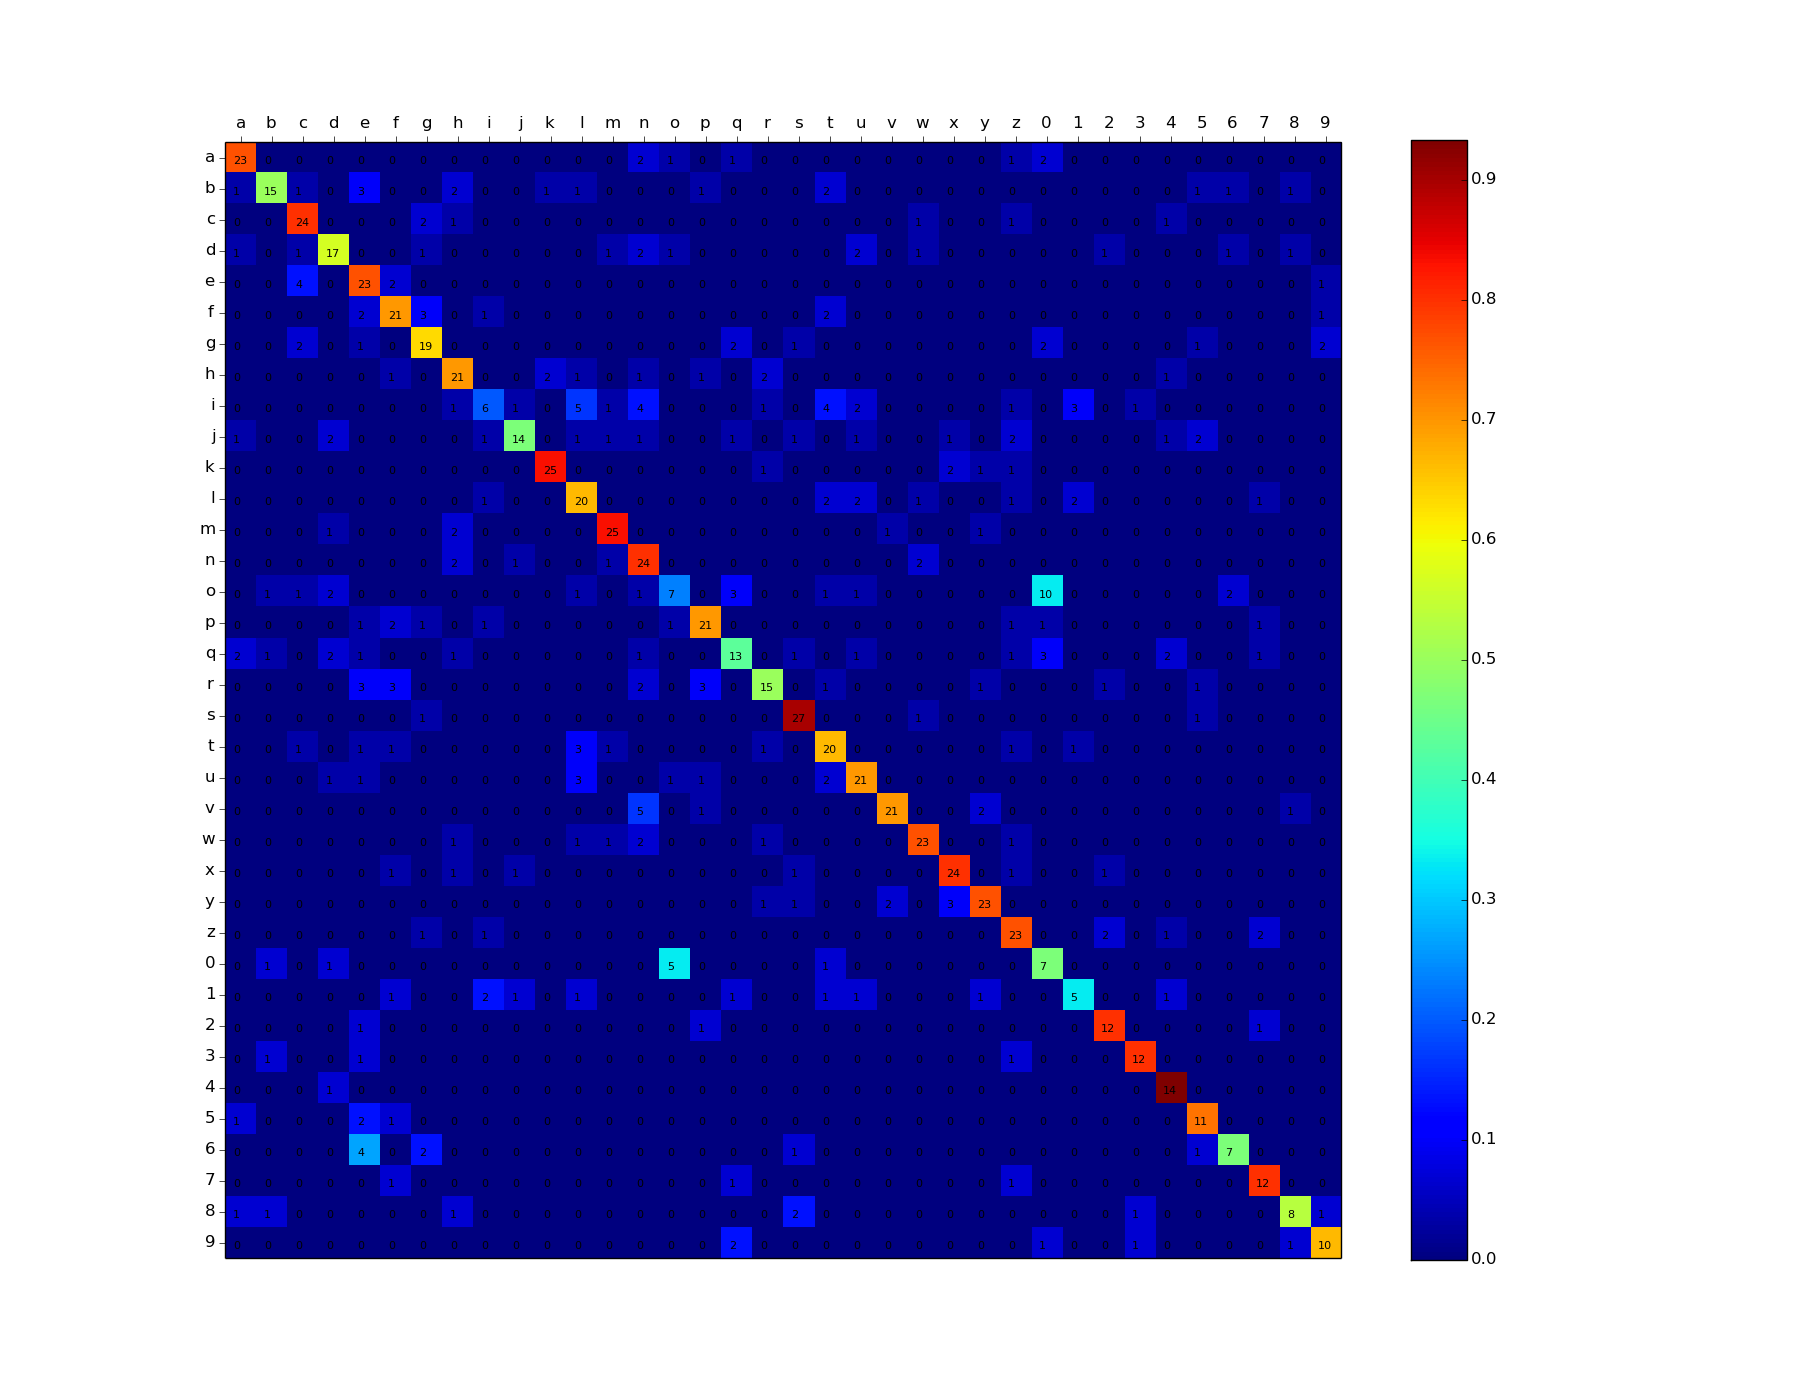
\includegraphics[scale=0.4]{img/resultados/mixtas/best_mean_matrix_Alpha0,01_4080-8_ins.png}}
				\caption[Matriz de correlación ``case insensitive'' para mixtas media]{Matriz de correlación del gráfico \ref{fig: Mixtas-media-mejor} para el mejor resultado no teniendo en cuenta los caracteres en mayúscula.}
				\label{fig: MatrizIns-Mixtas-media-mejor}
			\end{figure}

